\pagestyle{fancy}

In this chapter, the traditional methods of particles reconstruction and identification (without use of ML) are described.

%%%%%%%%%%%%%%%%% TOF
\section{Particle identification using the time-of-flight method}\thispagestyle{fancy}



The time-of-flight method (TOF) allows to differentiate between the groups of particles such as pions, kaons, and protons (positrons). Using the reconstructed:
\begin{itemize}
    \item momentum ($p$) and charge ($q$) (from the \textbf{STS} and \textbf{MVD} detectors) 
    \item time of flight ($t$) and length of the track in the detector ($L$) (from the \textbf{TOF} detector)
\end{itemize} the mass-squared of a reconstructed particle can be calculated following the formula:
\begin{equation}
    m^2 = \frac{p^2}{c^2} \cdot \left(\frac{c^2t^2}{L^2} - 1 \right)
    \label{msquared}
\end{equation}
where  $c$ - velocity of light in vacuum. Making a 2D plot, showing $m^2$ on the \emph{y}-axis, and $p\cdot q$ on the \emph{x}-axis, we receive a plot such as in Figure \ref{tof plot}. To further differentiate between the groups of the particles, Gaussian functions can be fitted to the distributions of the mass-squared. 
However, the last step is a non-trivial task, causing the majority of the inaccuracy, especially for particles whose mass-squared is far from the mean $m^2$ value of their group. 
While several solutions to this problem, such as multidimensional fitting (using more reconstructed variables) exist, the application of ML algorithms will be discussed in this work. 

Other groups of particles such as e.g., muons and electrons, can also be reconstructed using the data from other detectors ( MUCH and RICH respectively), but it goes beyond the scope of this thesis.

\begin{figure}[H]
    \centering
    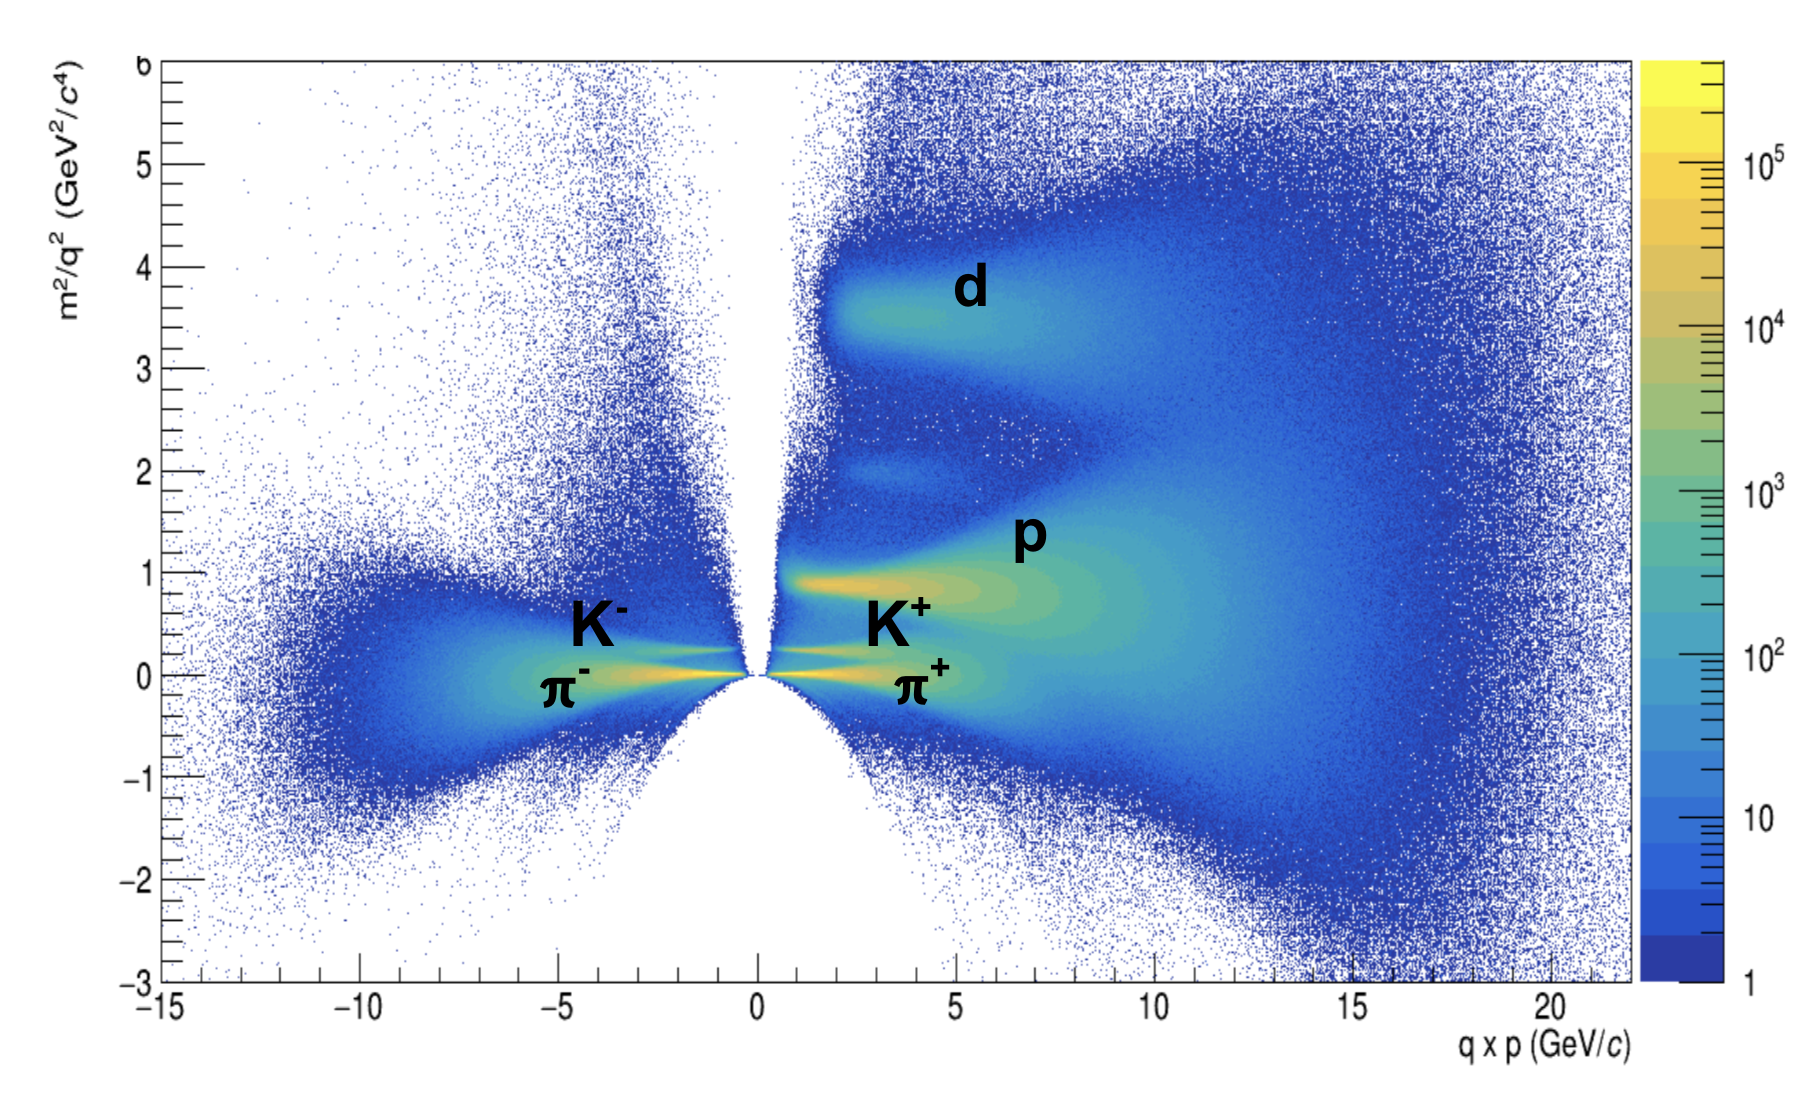
\includegraphics[width=.9\textwidth]{inz_szablon_new/img/tof_plot.pdf}
    \caption{2D TOF plot with pions, kaons, and protons shown}
    \label{tof plot}
\end{figure}
    

%%%%%%%%%%%%%%%%% KFPF
\section{Short-lived particles reconstruction}

Short-lived particles like $\Lambda^0$, and \PKshort have a neutral charge, therefore they cannot be detected directly using e.g., the TOF method. However, we can reconstruct these particles by investigating their \emph{daughter particles} - particles coming from their decays. For example, in the main decay mode (66.7\%) a K-short particle decays into a positive and negative pion (Figure \ref{ks decay}). Using i.e. the STS, we can reconstruct the tracks of pions (identified earlier using e.g., TOF method) coming from this decay, and thus reconstruct the K-short particle.

\begin{figure}[H]
\centering
    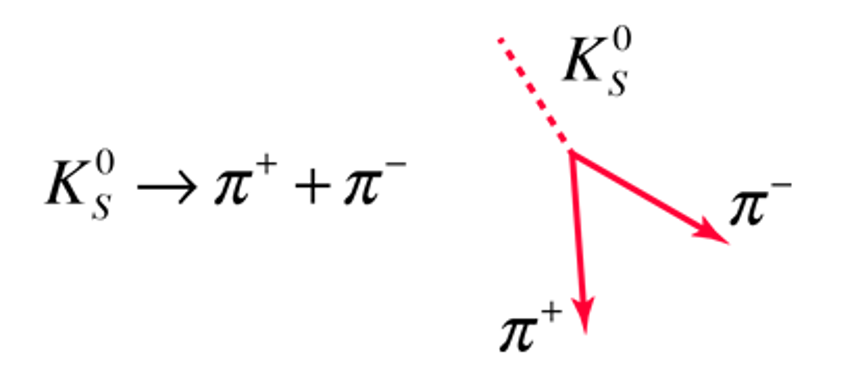
\includegraphics[width=.4\textwidth]{img/kdecay1.png}
    \caption{\PKshort main decay mode \cite{kdecay1}}
    \label{ks decay}
\end{figure}

In order to do so, the \textbf{KFParticleFinder} was developed \cite{kfp}. It is an on-line optimized particle reconstruction package based on Kalman Filter mathematics. It finds pairs of positive and negative pions (in the \PKshort case) which could be a result of the \emph{mother} particle's decay.
%------------------------- PFSimple
\subsection{PFSimple}
For offline selection optimization and analysis, \textbf{PFSimple} package was created \cite{lubynets}. Using it, one can optimize selection criteria to differentiate between:
\begin{itemize}
    \item \textbf{signal} - pion pairs created in K-short decay
    \item \textbf{background} - pions pairs returned by KFParticleFinder which are not the result of K-short decay
\end{itemize}
Also, PFSimple returns these attributes of each reconstructed particle (visualised on Figure \ref{pfsimple}):
\begin{itemize}
    \item \textbf{L/$\Delta$L} - distance between primary and secondary vertex divided over its error
    \item \textbf{DCA} - distance of closest approach between pion tracks
    \item \textbf{$\chi^2$ geo} - dimensionless distance of closest approach between pion tracks
    \item \textbf{$\chi^2$ topo} - dimensionless distance of closest approach between extrapolated kaon trajectory and primary vertex
    \item \textbf{$\chi^2$ prim} - dimensionless distance between extrapolated secondary track and primary vertex
    \item \textbf{$\cos(\alpha)$} - cosine of angle between pion and K-short momenta
\end{itemize}
\begin{figure}[H]
    \centering
    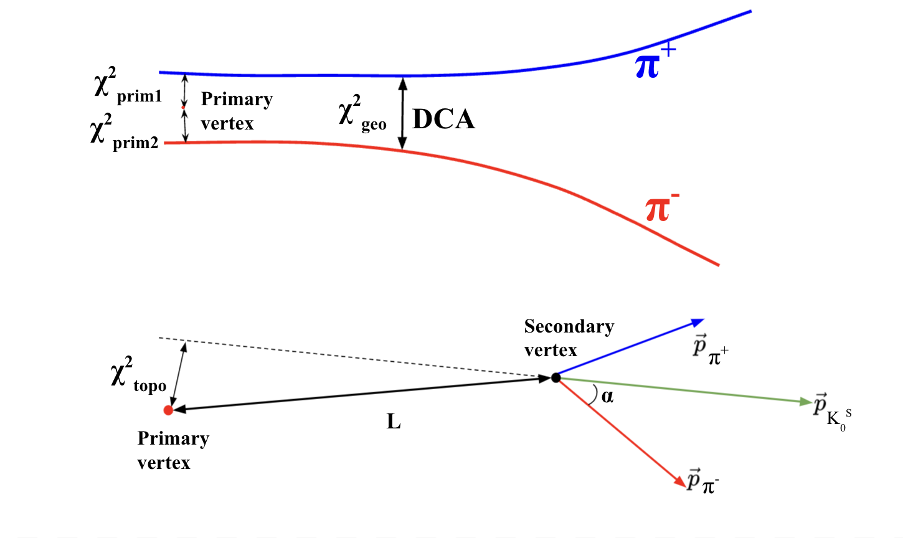
\includegraphics[width=.9\textwidth]{img/pfsimple_variables.png}
    \caption{Decay scheme and topological variables of a \PKshort decay in the PFSimple}
    \label{pfsimple}
\end{figure}
%------------------------- optimization of selection criteria
\subsubsection{Optimization of selection criteria}
As the KFParticle Finder (and PFSimple) return all the possible pion pairs, which could be a result of K-short decay,  some selection criteria need to be applied to differentiate between the signal and background.\\

The manual selection criteria can also be visualised with a decision tree (Figure \ref{manual tree}):
\begin{itemize}
    \item For each variable of a reconstructed particle, a conditional statement is being set
    \item If all conditions are fulfilled, a K-short candidate is treated as a signal  candidate
\end{itemize}

\begin{figure}[H]
    \centering
    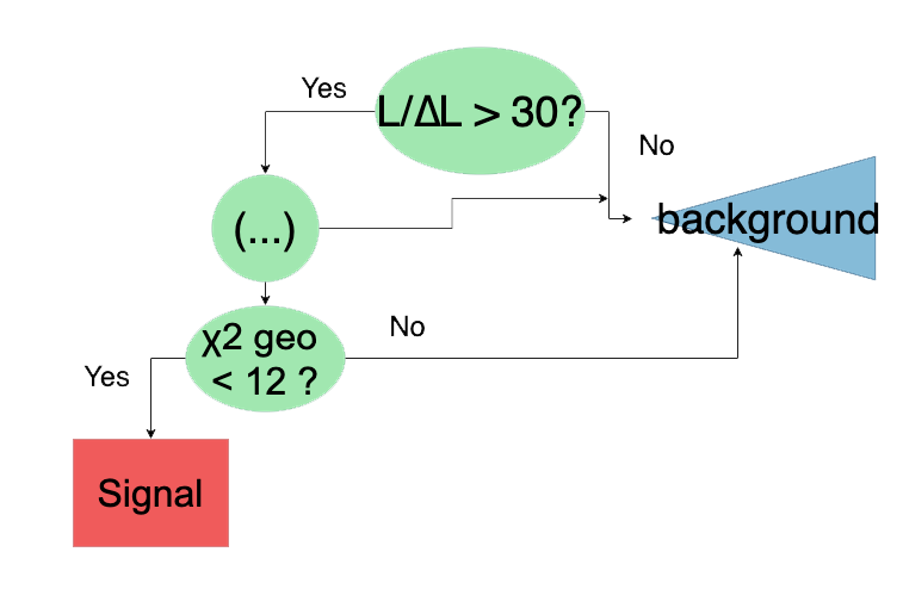
\includegraphics[width=.6\textwidth]{img/decision_tree.png}
    \caption{Example of a decision tree using manual selection criteria}
    \label{manual tree}
\end{figure}

The manual procedure for selection criteria optimization \cite{lubynets} is as follows:
\begin{enumerate}
    \item The goal is to suppress as much background and to preserve as much signal as possible 
    \item Plot distribution of signal and background for some variable (e.g., on Figure \ref{manual distributions}), and select a point above which all entries are considered as signal or background
    \item Repeat it for all the variables
\end{enumerate}
\begin{figure}[H]
    \centering
    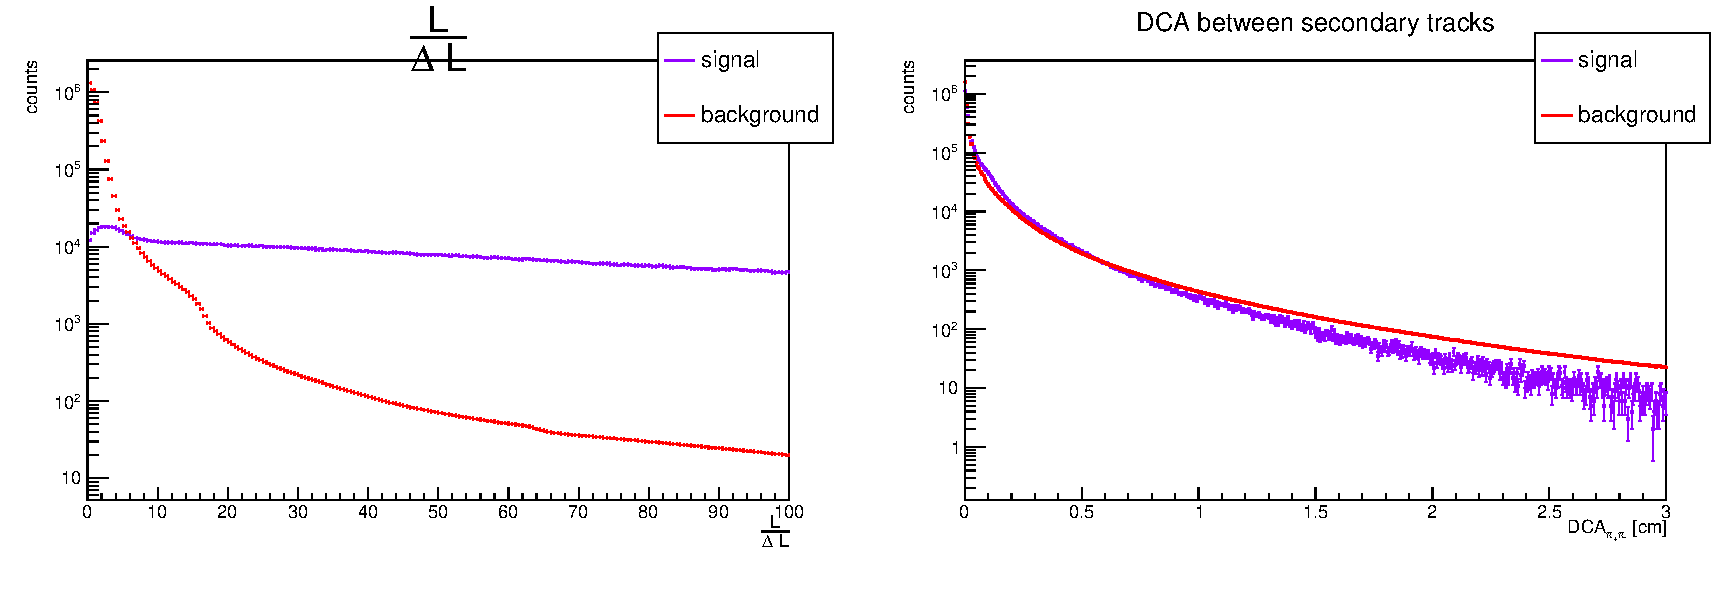
\includegraphics[width=1\textwidth]{img/pfsimple_distributions.pdf}
     \caption{Example of distributions to be checked with the manual selection criteria optimization}
     \label{manual distributions}
\end{figure}

However, this task is non-automatized (must be repeated for each particle), collision simulating model dependent, and only linear (as one variable at a time is used). In this work, the application of ML algorithm for the optimization of selection criteria will be discussed.
